\begin{figure}[H]
\centering
\subfigure{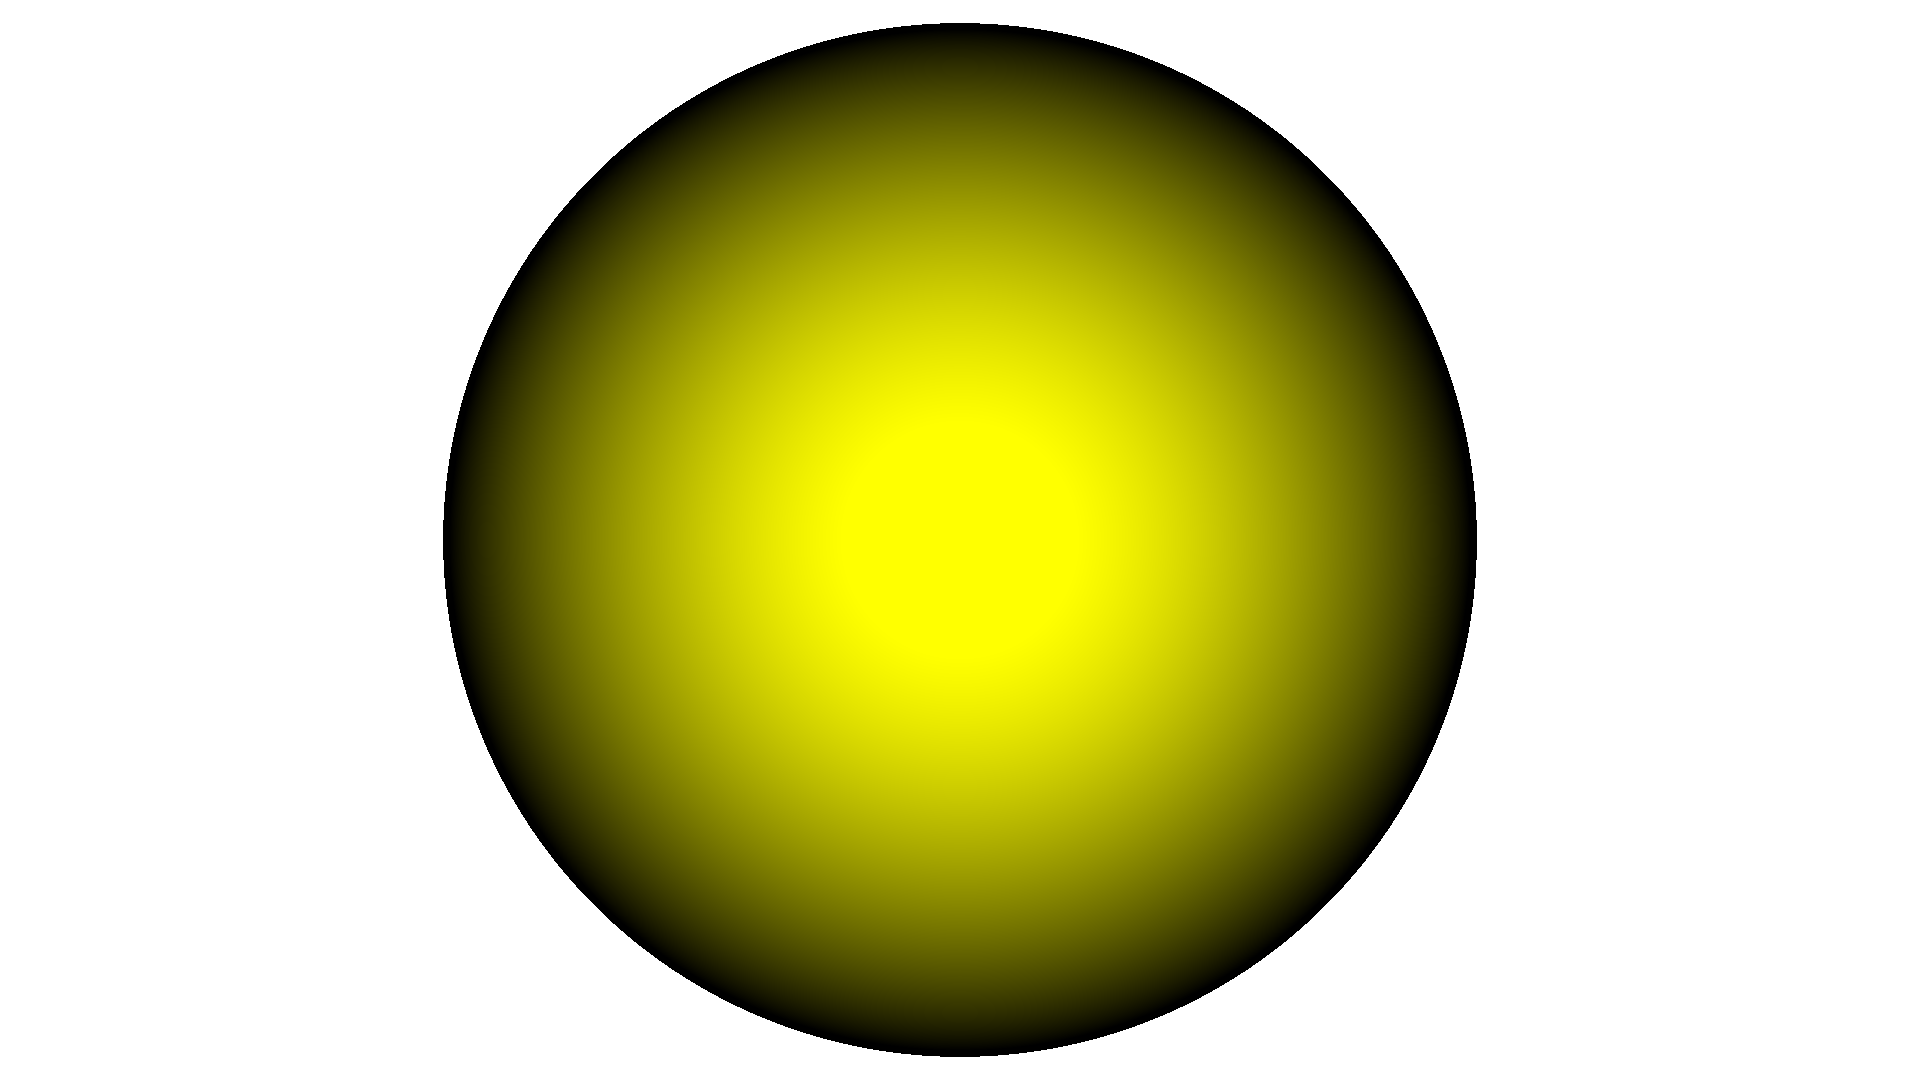
\includegraphics[width=0.3\textwidth]{chapters/ch3/img/diffuse/direct_0.png}}
\subfigure{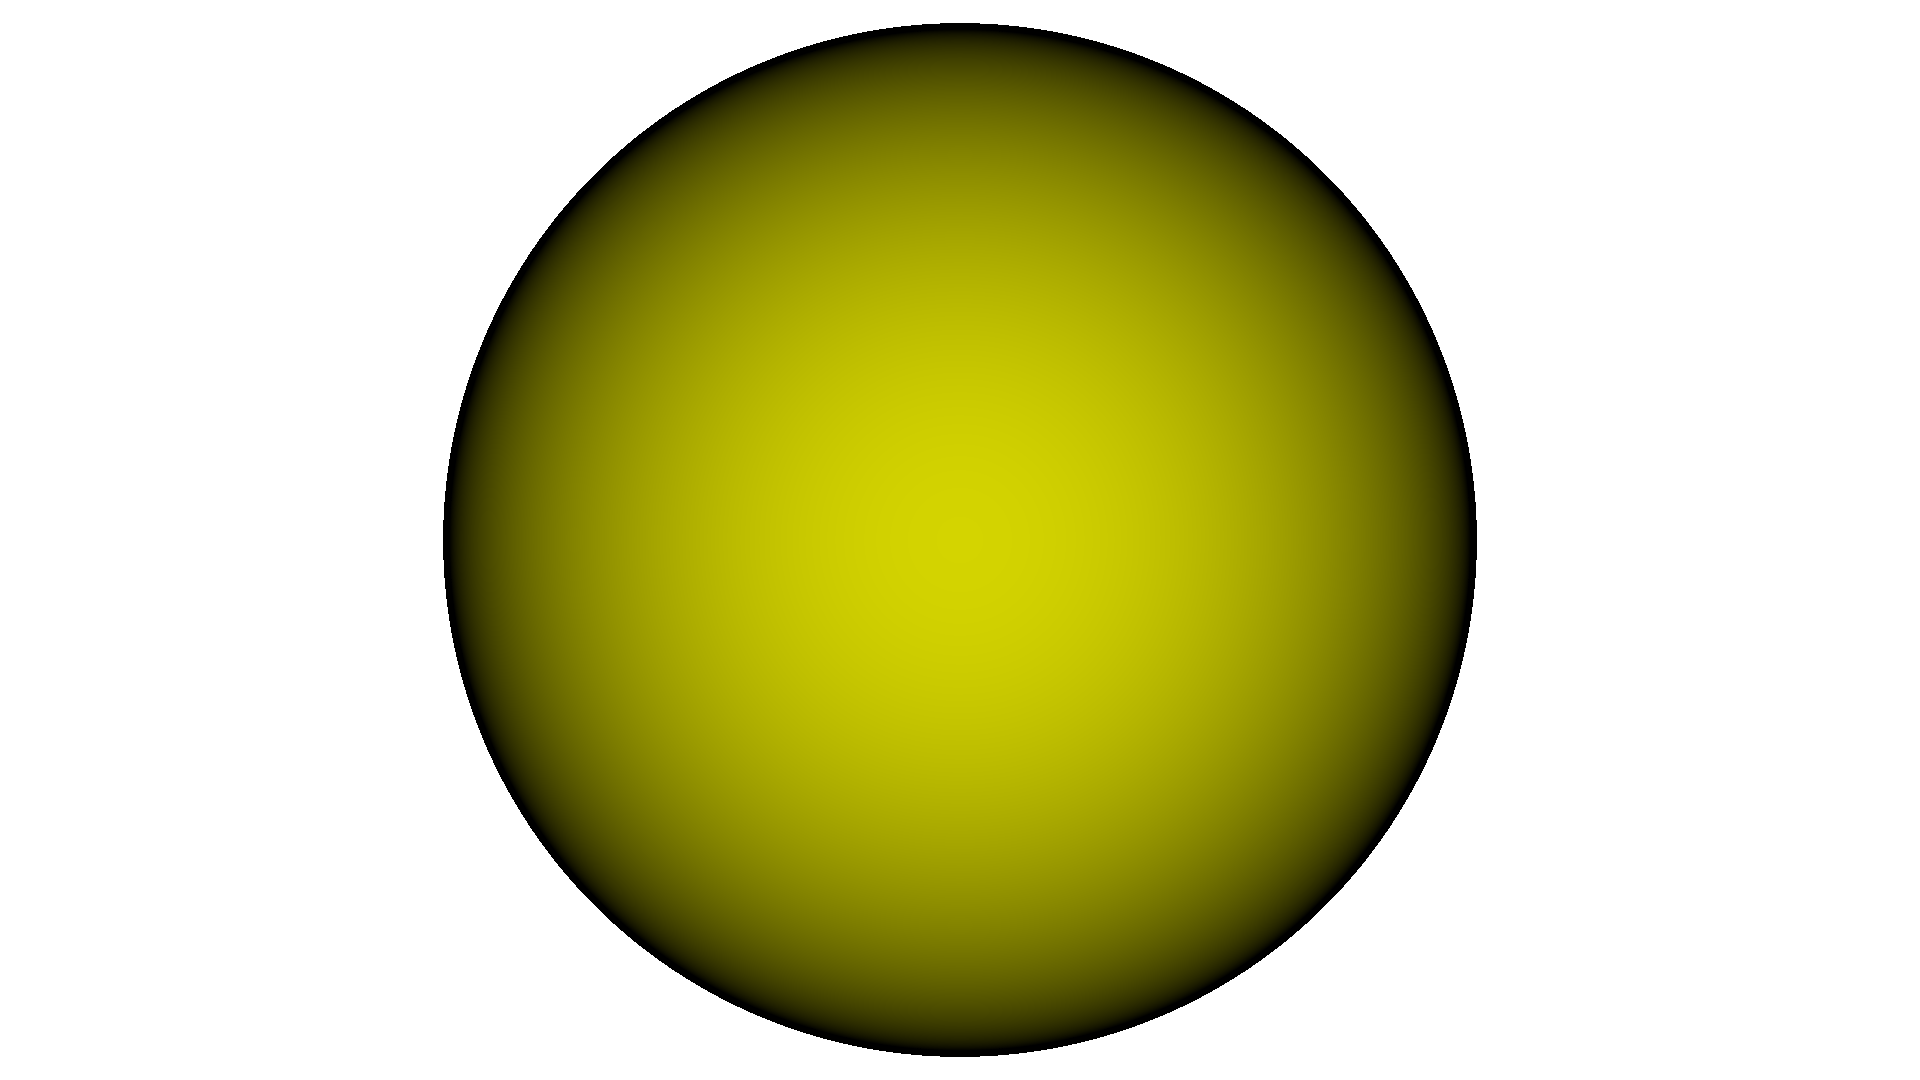
\includegraphics[width=0.3\textwidth]{chapters/ch3/img/diffuse/direct_025.png}}
\subfigure{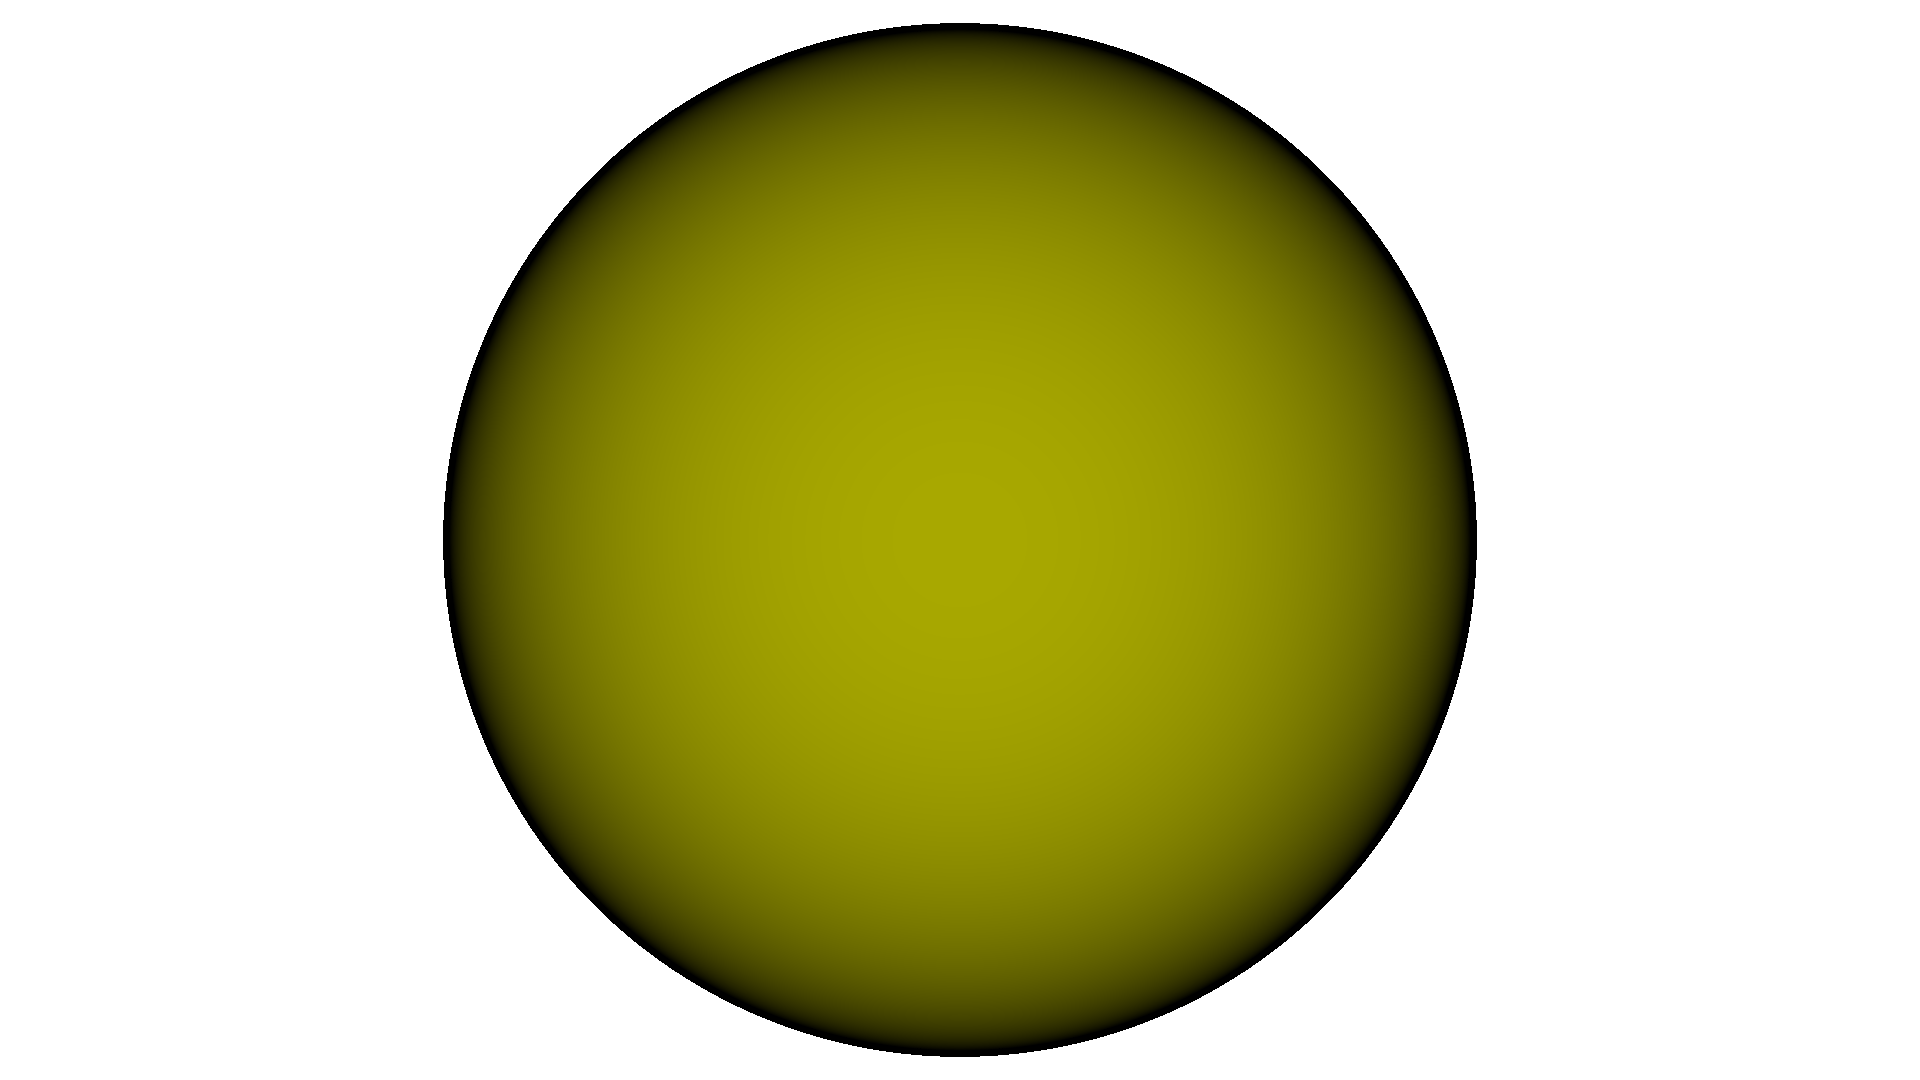
\includegraphics[width=0.3\textwidth]{chapters/ch3/img/diffuse/direct_1.png}}

\subfigure{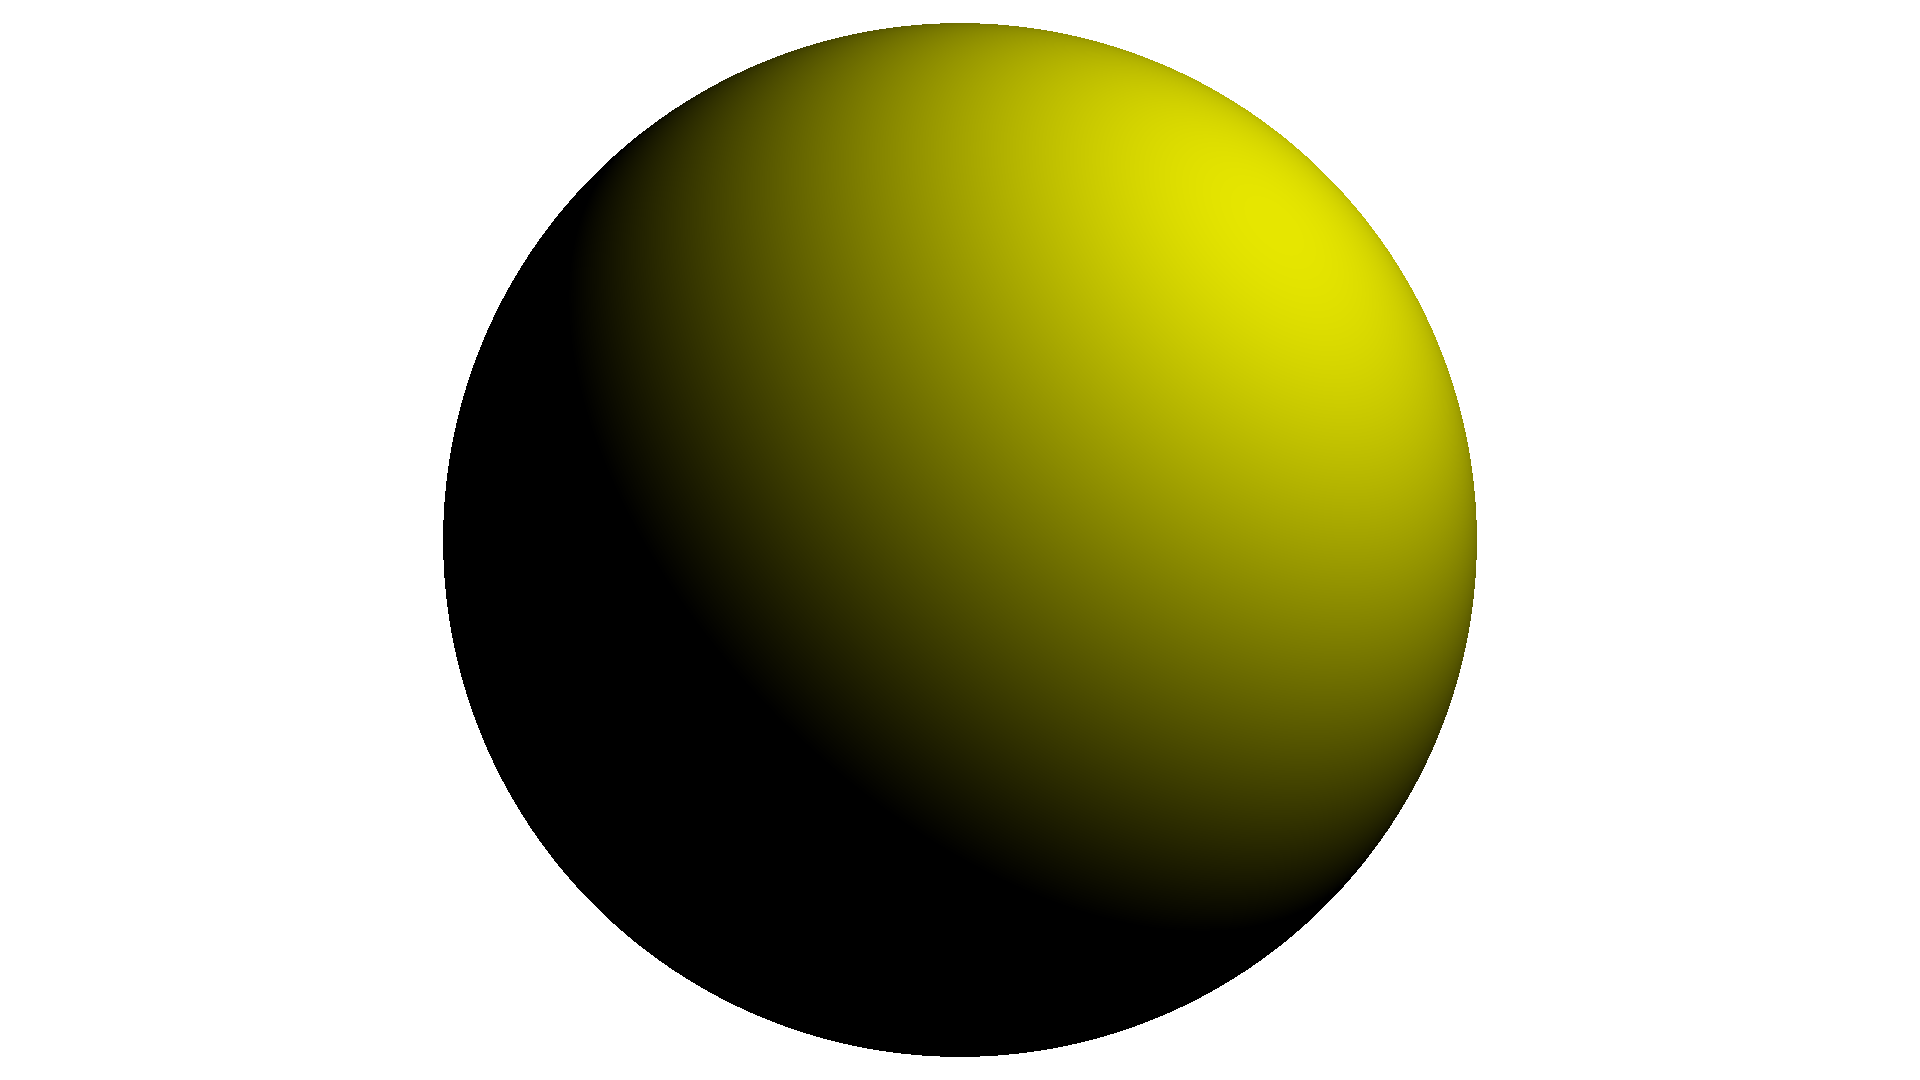
\includegraphics[width=0.3\textwidth]{chapters/ch3/img/diffuse/angle_0.png}}
\subfigure{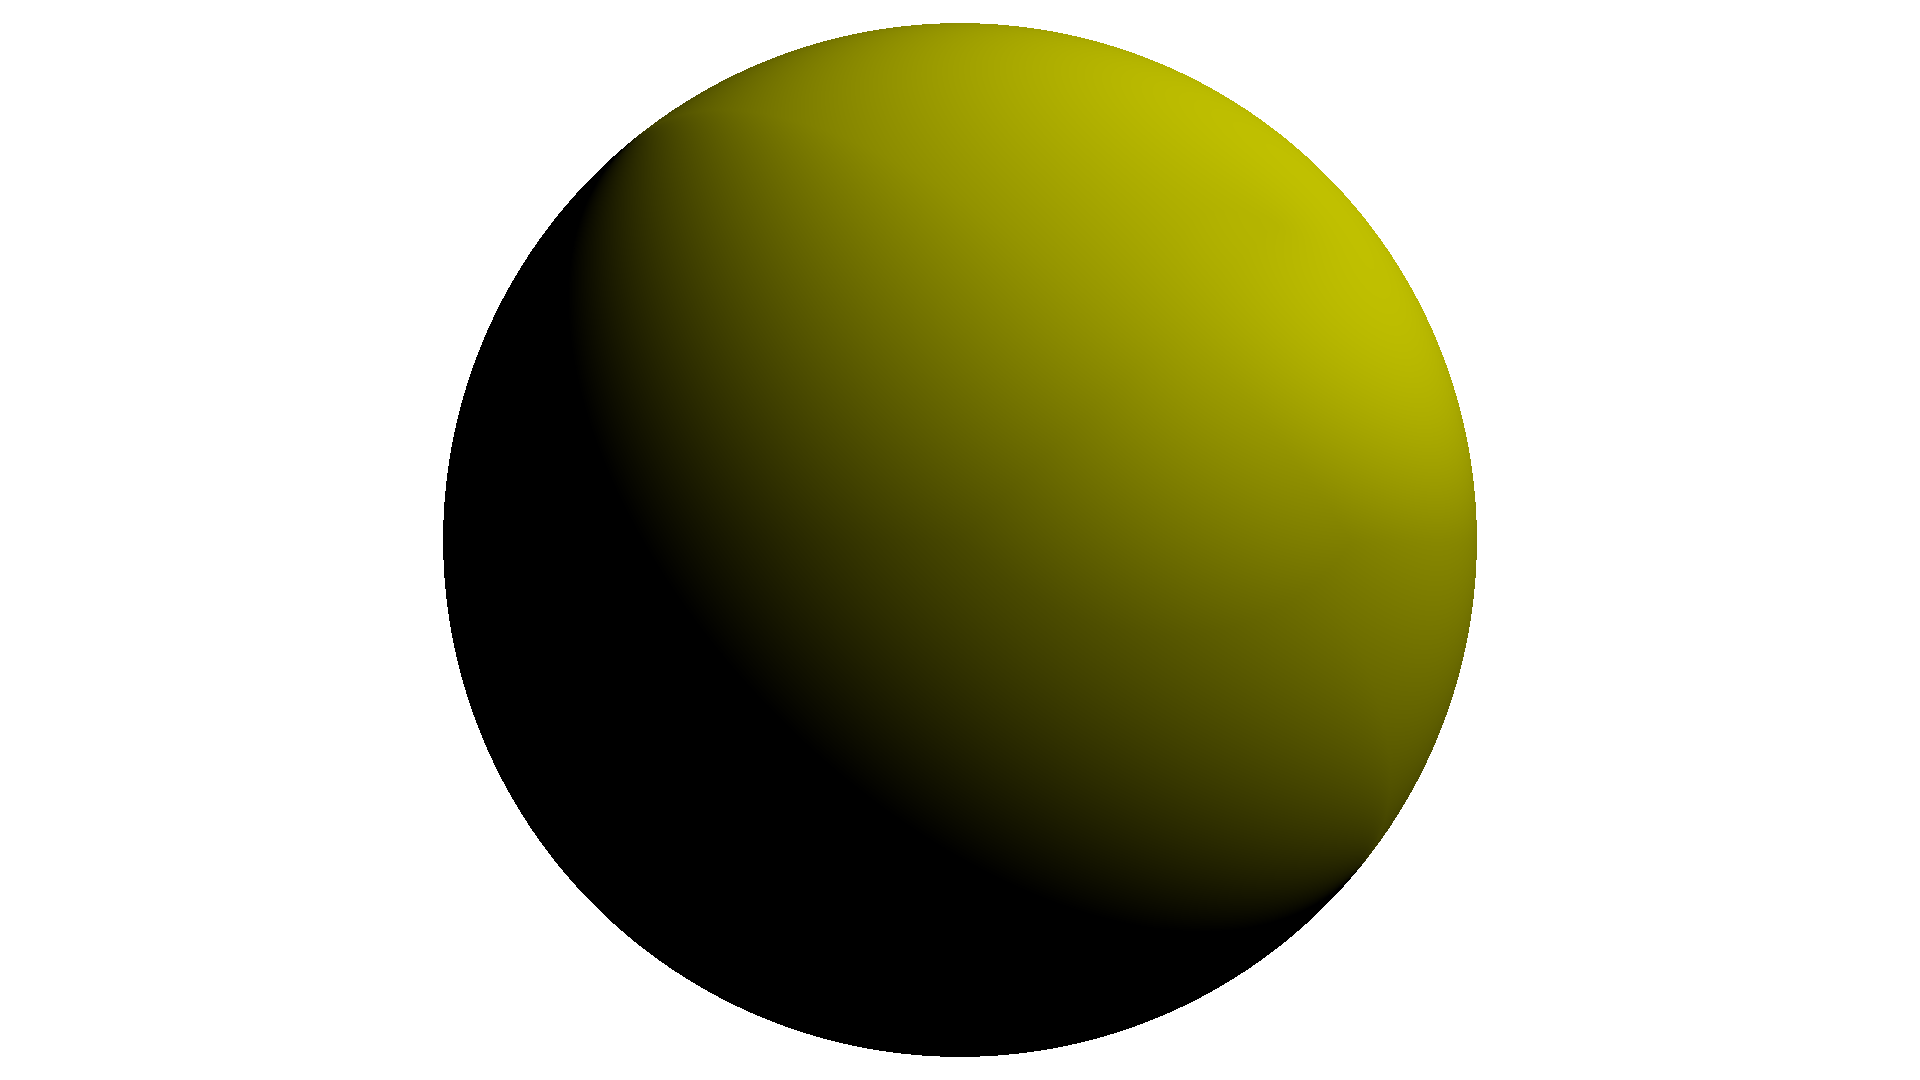
\includegraphics[width=0.3\textwidth]{chapters/ch3/img/diffuse/angle_025.png}}
\subfigure{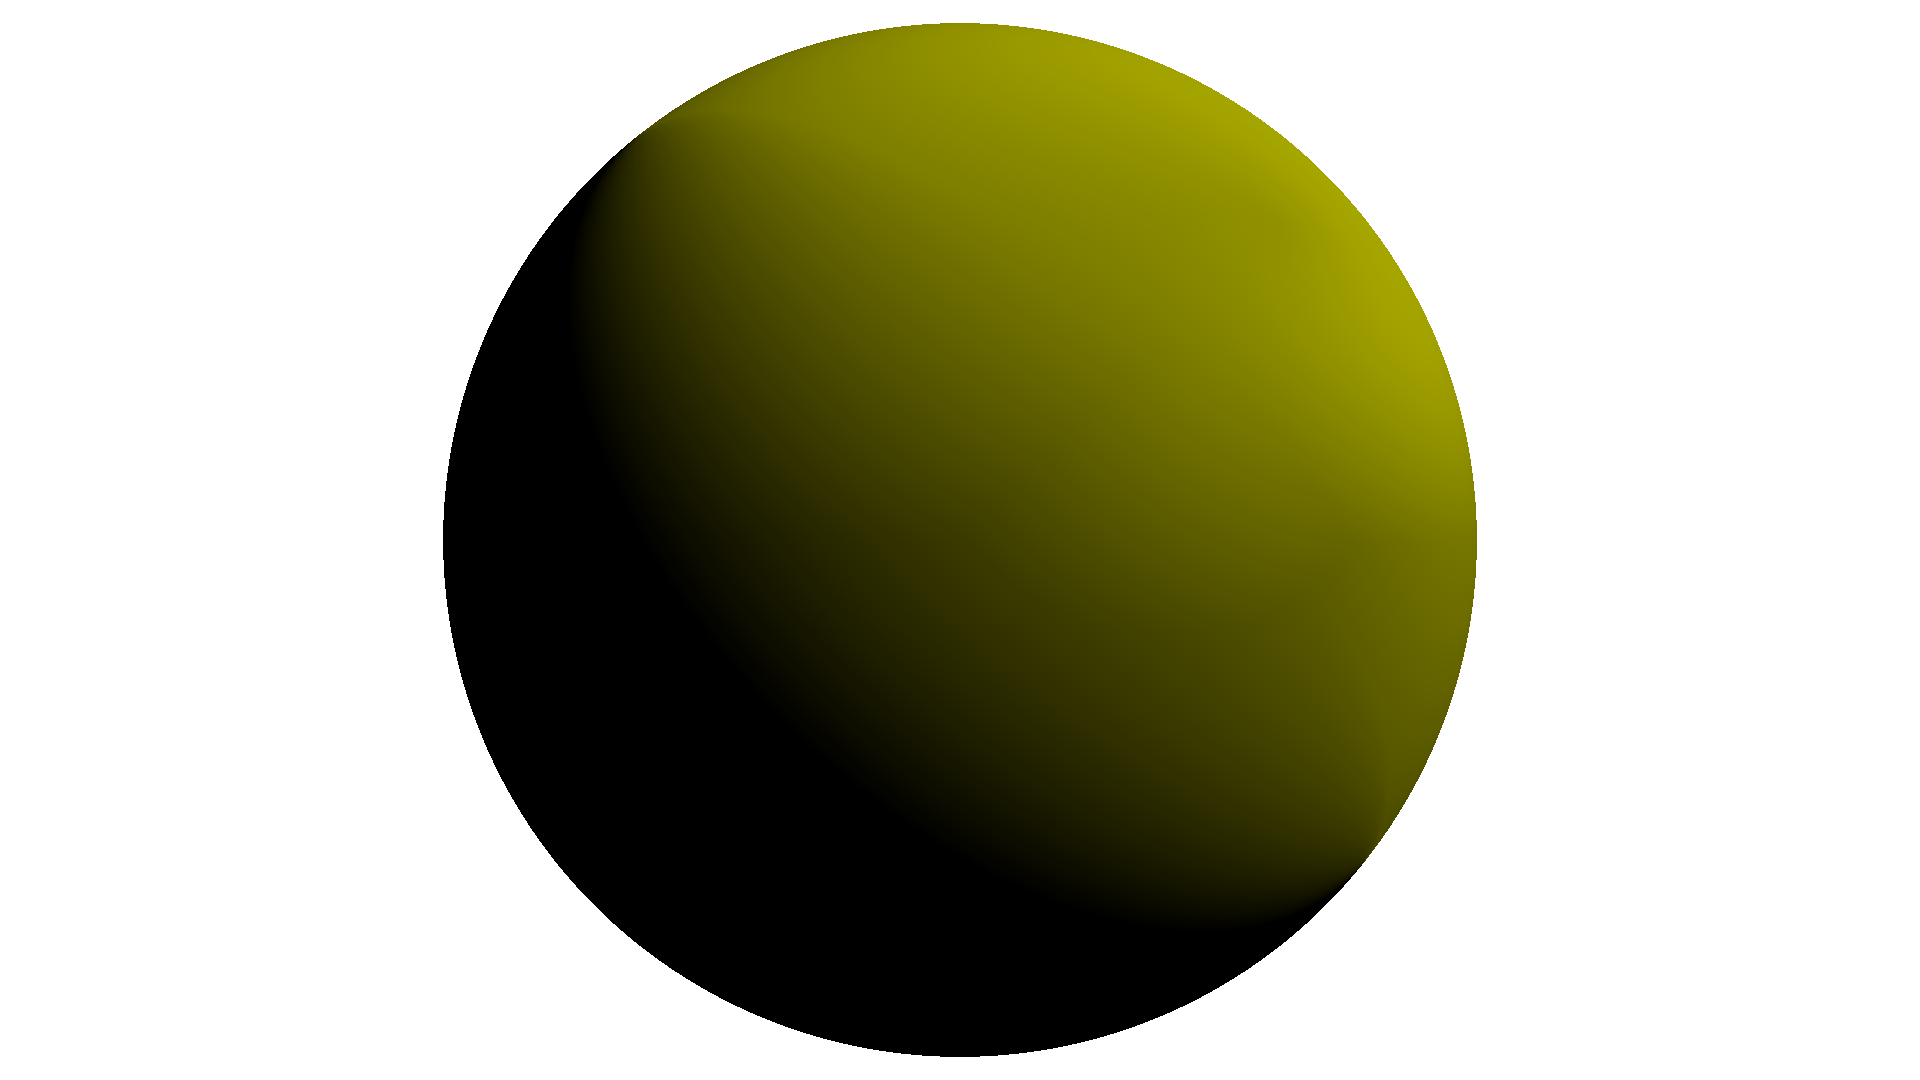
\includegraphics[width=0.3\textwidth]{chapters/ch3/img/diffuse/angle_1.png}}

\caption[Oświetlenie powierzchni odbijającej światło całkowicie w sposób rozproszony zgodnie z modelem Orena-Nayara]{Oświetlenie powierzchni odbijającej światło całkowicie w sposób rozproszony zgodnie z modelem Orena-Nayara. Górny wiersz odpowiada sytuacji, gdy kierunek obserwacji $\vec{d}$ oraz kierunek światła $\overrightarrow{l_{dir}}$ są identyczne i przechodzą przez środek oświetlanej kuli. W~dolnym wierszu wspomniane kierunki nie pokrywają się. Kolejne kolumny~(od lewej do prawej) odpowiadają różnym wartościom współczynnika szorstkości materiału $\sigma^2\in\lbrace 0; 0,25; 1 \rbrace$, wraz ze wzrostem którego następuje coraz większe zrównanie jasności oświetlanej powierzchni}
\label{ch3:img:diffuse_params}
\end{figure}